\documentclass[10pt]{article}
\usepackage{amsmath}
\usepackage{amsthm}
\usepackage{amsfonts}
\usepackage{dsfont}
\usepackage{amssymb}
\usepackage{latexsym}
\usepackage{tensor}
%\usepackage{epsfig}
\usepackage{graphicx}
\usepackage{xfrac}
\usepackage{tikz}
\usetikzlibrary{cd}
%\usepackage[dvips]{graphicx}
\graphicspath{ {images/} }
\usepackage{pict2e}
\usepackage[font={small}]{caption}

\newcommand{\mnote}[1]{${}^*$\marginpar{\footnotesize ${}^*$#1}}
\linespread{1.065}

\makeatletter

\setlength\@tempdima  {5.5in}
\addtolength\@tempdima {-\textwidth}
\addtolength\hoffset{-0.5\@tempdima}
\setlength{\textwidth}{5.5in}
\setlength{\textheight}{8.75in}
\addtolength\voffset{-0.625in}

\makeatother

\makeatletter 
\@addtoreset{equation}{section}
\makeatother


\renewcommand{\theequation}{\thesection.\arabic{equation}}

\theoremstyle{plain}
\newtheorem{theorem}[equation]{Theorem}
\newtheorem{corollary}[equation]{Corollary}
\newtheorem{lemma}[equation]{Lemma}
\newtheorem{proposition}[equation]{Proposition}
\newtheorem{conjecture}[equation]{Conjecture}
\newtheorem{fact}[equation]{Fact}
\newtheorem{facts}[equation]{Facts}
\newtheorem*{theoremA}{Theorem A}
\newtheorem*{theoremB}{Theorem B}
\newtheorem*{theoremC}{Theorem C}
\newtheorem*{theoremD}{Theorem D}
\newtheorem*{theoremE}{Theorem E}
\newtheorem*{theoremF}{Theorem F}
\newtheorem*{theoremG}{Theorem G}
\newtheorem*{theoremH}{Theorem H}

\theoremstyle{definition}
\newtheorem{definition}[equation]{Definition}
\newtheorem{definitions}[equation]{Definitions}
%\theoremstyle{remark}

\newtheorem{remark}[equation]{Remark}
\newtheorem{remarks}[equation]{Remarks}
\newtheorem{exercise}[equation]{Exercise}
\newtheorem{example}[equation]{Example}
\newtheorem{examples}[equation]{Examples}
\newtheorem{notation}[equation]{Notation}
\newtheorem{question}[equation]{Question}
\newtheorem{assumption}[equation]{Assumption}
\newtheorem*{claim}{Claim}
\newtheorem{answer}[equation]{Answer}
%%%%%% letters %%%%

\newcommand{\fA}{\mathfrak{A}}
\newcommand{\fB}{\mathfrak{B}}
\newcommand{\fC}{\mathfrak{C}}
\newcommand{\fD}{\mathfrak{D}}
\newcommand{\fE}{\mathfrak{E}}
\newcommand{\fF}{\mathfrak{F}}
\newcommand{\fG}{\mathfrak{G}}
\newcommand{\fH}{\mathfrak{H}}
\newcommand{\fI}{\mathfrak{I}}
\newcommand{\fJ}{\mathfrak{J}}
\newcommand{\fK}{\mathfrak{K}}
\newcommand{\fL}{\mathfrak{L}}
\newcommand{\fM}{\mathfrak{M}}
\newcommand{\fN}{\mathfrak{N}}
\newcommand{\fO}{\mathfrak{O}}
\newcommand{\fP}{\mathfrak{P}}
\newcommand{\fQ}{\mathfrak{Q}}
\newcommand{\fR}{\mathfrak{R}}
\newcommand{\fS}{\mathfrak{S}}
\newcommand{\fT}{\mathfrak{T}}
\newcommand{\fU}{\mathfrak{U}}
\newcommand{\fV}{\mathfrak{V}}
\newcommand{\fW}{\mathfrak{W}}
\newcommand{\fX}{\mathfrak{X}}
\newcommand{\fY}{\mathfrak{Y}}
\newcommand{\fZ}{\mathfrak{Z}}

\newcommand{\fa}{\mathfrak{a}}
\newcommand{\fb}{\mathfrak{b}}
\newcommand{\fc}{\mathfrak{c}}
\newcommand{\fd}{\mathfrak{d}}
\newcommand{\fe}{\mathfrak{e}}
\newcommand{\ff}{\mathfrak{f}}
\newcommand{\fg}{\mathfrak{g}}
\newcommand{\fh}{\mathfrak{h}}
%\newcommand{\fi}{\mathfrak{i}}

\newcommand{\fj}{\mathfrak{j}}
\newcommand{\fk}{\mathfrak{k}}
\newcommand{\fl}{\mathfrak{l}}
\newcommand{\fm}{\mathfrak{m}}
\newcommand{\fn}{\mathfrak{n}}
\newcommand{\fo}{\mathfrak{o}}
\newcommand{\fp}{\mathfrak{p}}
\newcommand{\fq}{\mathfrak{q}}
\newcommand{\fr}{\mathfrak{r}}
\newcommand{\fs}{\mathfrak{s}}
\newcommand{\ft}{\mathfrak{t}}
\newcommand{\fu}{\mathfrak{u}}
\newcommand{\fv}{\mathfrak{v}}
\newcommand{\fw}{\mathfrak{w}}
\newcommand{\fx}{\mathfrak{x}}
\newcommand{\fy}{\mathfrak{y}}
\newcommand{\fz}{\mathfrak{z}}

\newcommand{\bi}{\textbf{i}}
\newcommand{\bj}{\textbf{j}}
\newcommand{\bk}{\textbf{k}}

\newcommand{\sA}{\mathcal{A}\,}
\newcommand{\sB}{\mathcal{B}\,}
\newcommand{\sC}{\mathcal{C}}
\newcommand{\sD}{\mathcal{D}\,}
\newcommand{\sE}{\mathcal{E}\,}
\newcommand{\sF}{\mathcal{F}\,}
\newcommand{\sG}{\mathcal{G}\,}
\newcommand{\sH}{\mathcal{H}}
\newcommand{\sI}{\mathcal{I}\,}
\newcommand{\sJ}{\mathcal{J}\,}
\newcommand{\sK}{\mathcal{K}\,}
\newcommand{\sL}{\mathcal{L}\,}
\newcommand{\sM}{\mathcal{M}\,}
\newcommand{\sN}{\mathcal{N}}
\newcommand{\sO}{\mathcal{O}}
\newcommand{\sP}{\mathcal{P}\,}
\newcommand{\sQ}{\mathcal{Q}\,}
\newcommand{\sR}{\mathcal{R}}
\newcommand{\sS}{\mathcal{S}}
\newcommand{\sT}{\mathcal{T}\,}
\newcommand{\sU}{\mathcal{U}\,}
\newcommand{\sV}{\mathcal{V}\,}
\newcommand{\sW}{\mathcal{W}\,}
\newcommand{\sX}{\mathcal{X}\,}
\newcommand{\sY}{\mathcal{Y}\,}
\newcommand{\sZ}{\mathcal{Z}\,}

\newcommand{\IA}{\mathbb{A}}
\newcommand{\IB}{\mathbb{B}}
\newcommand{\IC}{\mathbb{C}}
\newcommand{\ID}{\mathbb{D}}
\newcommand{\IE}{\mathbb{E}}
\newcommand{\IF}{\mathbb{F}}
\newcommand{\IG}{\mathbb{G}}
\newcommand{\IH}{\mathbb{H}}
\newcommand{\II}{\mathbb{I}}
\newcommand{\IK}{\mathbb{K}}
\newcommand{\IL}{\mathbb{L}}
\newcommand{\IM}{\mathbb{M}}
\newcommand{\IN}{\mathbb{N}}
\newcommand{\IO}{\mathbb{O}}
\newcommand{\IP}{\mathbb{P}}
\newcommand{\IQ}{\mathbb{Q}}
\newcommand{\IR}{\mathbb{R}}
\newcommand{\IS}{\mathbb{S}}
\newcommand{\IT}{\mathbb{T}}
\newcommand{\IU}{\mathbb{U}}
\newcommand{\IV}{\mathbb{V}}
\newcommand{\IW}{\mathbb{W}}
\newcommand{\IX}{\mathbb{X}}
\newcommand{\IY}{\mathbb{Y}}
\newcommand{\IZ}{\mathbb{Z}}

 \newcommand{\tA}{\mathrm {A}}
 \newcommand{\tB}{\mathrm {B}}
 \newcommand{\tC}{\mathrm {C}}
 \newcommand{\tD}{\mathrm {D}}
 \newcommand{\tE}{\mathrm {E}}
 \newcommand{\tF}{\mathrm {F}}
 \newcommand{\tG}{\mathrm {G}}
 \newcommand{\tH}{\mathrm {H}}
 \newcommand{\tI}{\mathrm {I}}
 \newcommand{\tJ}{\mathrm {J}}
 \newcommand{\tK}{\mathrm {K}}
 \newcommand{\tL}{\mathrm {L}}
 \newcommand{\tM}{\mathrm {M}}
 \newcommand{\tN}{\mathrm {N}}
 \newcommand{\tO}{\mathrm {O}}
 \newcommand{\tP}{\mathrm {P}}
 \newcommand{\tQ}{\mathrm {Q}}
 \newcommand{\tR}{\mathrm {R}}
 \newcommand{\tS}{\mathrm {S}}
 \newcommand{\tT}{\mathrm {T}}
 \newcommand{\tU}{\mathrm {U}}
 \newcommand{\tV}{\mathrm {V}}
 \newcommand{\tW}{\mathrm {W}}
 \newcommand{\tX}{\mathrm {X}}
 \newcommand{\tY}{\mathrm {Y}}
 \newcommand{\tZ}{\mathrm {Z}}
%%%%%%% macros %%%%%

%% my definitions %%%

\newcommand{\End}{\mathrm{End}}
\newcommand{\tr}{\mathrm{tr}}
%\newcommand{\ind}{\mathrm{ind}}

\renewcommand{\index}{\mathrm{index \,}}
\newcommand{\Hom}{\mathrm{Hom}}
\newcommand{\Aut}{\mathrm{Aut}}
\newcommand{\Trace}{\mathrm{Trace}\,}
\newcommand{\Res}{\mathrm{Res}\,}
\newcommand{\rank}{\mathrm{rank}}
%\renewcommand{\dim}{\mathrm{dim}}

\renewcommand{\deg}{\mathrm{deg}}
\newcommand{\spin}{\rm Spin}
\newcommand{\Spin}{\rm Spin}
\newcommand{\erfc}{\rm erfc\,}
\newcommand{\sgn}{{\rm sgn\,}}
\newcommand{\Spec}{\rm Spec\,}
\newcommand{\diag}{\rm diag\,}
\newcommand{\Fix}{\mathrm{Fix}}
\newcommand{\Ker}{\mathrm{Ker \,}}
\newcommand{\Coker}{\mathrm{Coker \,}}
\newcommand{\Sym}{\mathrm{Sym \,}}
\newcommand{\Hess}{\mathrm{Hess \,}}
\newcommand{\grad}{\mathrm{grad \,}}
\newcommand{\Center}{\mathrm{Center}}
\newcommand{\Lie}{\mathrm{Lie}}


\newcommand{\ch}{\rm ch} % Chern Character

\newcommand{\rk}{\rm rk} 
%\renewcommand{\c}{\rm c}  % Chern class

\newcommand{\sign}{\rm sign}
\renewcommand\dim{{\rm dim\,}}
\renewcommand\det{{\rm det\,}}
\newcommand{\dimKrull}{{\rm Krulldim\,}}
\newcommand\Rep{\mathrm{Rep}}
\newcommand\Hilb{\mathrm{Hilb}}
\newcommand\vol{\mathrm{vol}}

\newcommand\QED{\hfill $\Box$} %{\bf QED}} 

\newcommand\Pf{\nonintend{\em Proof. }}


\newcommand\reals{{\mathbb R}} 
\newcommand\complexes{{\mathbb C}}
\renewcommand\Re{\mathrm Re}
\renewcommand\Im{\mathrm Im}
\newcommand\integers{{\mathbb Z}}
\newcommand\quaternions{{\mathbb H}}


\newcommand\iso{{\cong}} 
%\newcommand\tensor{{\otimes}}
\newcommand\Tensor{{\bigotimes}} 
\newcommand\union{\bigcup} 
\newcommand\onehalf{\frac{1}{2}}
%\newcommand\Sym[1]{{Sym^{#1}(\complexes^2)}}

\newcommand\lie[1]{{\mathfrak #1}} 
\renewcommand\fk{\mathfrak{K}}
\newcommand\smooth{\mathcal{C}^{\infty}}
\newcommand\trivial{{\mathbb I}}
\newcommand\widebar{\overline}

%%%%%Delimiters%%%%

\newcommand{\<}{\langle}
\renewcommand{\>}{\rangle}

%\renewcommand{\(}{\left(}
%\renewcommand{\)}{\right)}


%%%% Different kind of derivatives %%%%%

\newcommand{\delbar}{\bar{\partial}}
\newcommand{\pdu}{\frac{\partial}{\partial u}}
%\newcommand{\pd}[1][2]{\frac{\partial #1}{\partial #2}}

%%%%% Arrows %%%%%
%\renewcommand{\ra}{\rightarrow}                   % right arrow
%\newcommand{\lra}{\longrightarrow}              % long right arrow
%\renewcommand{\la}{\leftarrow}                    % left arrow
%\newcommand{\lla}{\longleftarrow}               % long left arrow
%\newcommand{\ua}{\uparrow}                     % long up arrow
%\newcommand{\na}{\nearrow}                      %  NE arrow
%\newcommand{\llra}[1]{\stackrel{#1}{\lra}}      % labeled long right arrow
%\newcommand{\llla}[1]{\stackrel{#1}{\lla}}      % labeled long left arrow
%\newcommand{\lua}[1]{\stackrel{#1}{\ua}}      % labeled  up arrow
%\newcommand{\lna}[1]{\stackrel{#1}{\na}}      % labeled long NE arrow

\newcommand{\into}{\hookrightarrow}
\newcommand{\tto}{\longmapsto}
\def\llra{\longleftrightarrow}

\def\d/{/\mspace{-6.0mu}/}
\newcommand{\git}[3]{#1\d/_{\mspace{-4.0mu}#2}#3}
\newcommand\zetahilb{\zeta_{{\text{Hilb}}}}
\def\Fy{\sF \mspace{-3.0mu} \cdot \mspace{-3.0mu} y}
\def\tv{\tilde{v}}
\def\tw{\tilde{w}}
\def\wt{\widetilde}
\def\wtilde{\widetilde}
\def\what{\widehat}

%%%%%%%%%%%%%%%%%%% Mark's definitions %%%%%%%%%%%%%%%%%%%%

\newcommand{\frakg}{\mbox{\frakturfont g}}
\newcommand{\frakk}{\mbox{\frakturfont k}}
\newcommand{\frakp}{\mbox{\frakturfont p}}
\newcommand{\q}{\mbox{\frakturfont q}}
\newcommand{\frakn}{\mbox{\frakturfont n}}
\newcommand{\frakv}{\mbox{\frakturfont v}}
\newcommand{\fraku}{\mbox{\frakturfont u}}
\newcommand{\frakh}{\mbox{\frakturfont h}}
\newcommand{\frakm}{\mbox{\frakturfont m}}
\newcommand{\frakt}{\mbox{\frakturfont t}}
\newcommand{\G}{\Gamma}
\newcommand{\g}{\gamma}
\newcommand{\fraka}{\mbox{\frakturfont a}}
\newcommand{\db}{\bar{\partial}}
\newcommand{\dbs}{\bar{\partial}^*}
\newcommand{\p}{\partial}

%%%%%%%%%%%%% new definitions for the positive mass paper %%%%%%%%%

\newcommand{\sperp}{{\scriptscriptstyle \perp}}

%%%%%%%%%%%%%%%%%%%%%%%



%%%%%%%%%%%%%%%%%%%%%%%%%%%%%%%%%%%%%%%%%%%%%


\tikzset{cross/.style={cross out, draw=black, fill=none, minimum size=2*(#1-\pgflinewidth), inner sep=0pt, outer sep=0pt}, cross/.default={2pt}}

%
\begin{document}
%

\title{Characterizing Rothe Diagrams}
\author{Ben Gillen and Jonathan Michala}

\date{\today}

\maketitle

\begin{abstract}
    We define five main properties that Rothe Diagrams fulfill: the southwest rule, dot rules, popping rules, numbering rules, step-out avoiding rule, and empty cell gap rule. 
    We prove that -- given an arbitrary bubble diagram -- three different subsets of these properties can fully determine a Rothe Diagram. 
    We also prove that the numbering and step-out rules can determine a Rothe Diagram from a set of ordered non-empty columns.
\end{abstract}

\section{Introduction}
Consider a permutation $w$ in $\fS_\infty$, the group of permutations on $\IZ^+$ with finitely many unfixed points.
For non-identity permutations, write a truncated $w = w_1w_2...w_n$, where $w_n$ is the last unfixed point.
The permutation correspondingly sends $i$ to $w_i$.
An \textbf{\textit{inversion}} of $w$ is a pair of indices $i < j$ such that $w_i > w_j$.
For example, if $w = 152869347$, then $w_4 = 8$ and $w_7 = 3$ would be an inversion.
One way to visualize inversions is with the \textbf{\textit{Rothe diagram}} of $w$, defined to be the following subset of cells in the first quadrant \cite{inversion}:
\begin{equation}
\ID(w) = \{(i,w_j) \colon i < j, w_i > w_j\} \subset \IZ^+ \times \IZ^+.
\end{equation}

Graphically, we represent cells in $\ID(w)$ by bubbles and use the convention that the $i$ coordinates are written on the vertical axis and the $w_j$ coordinates are written on the horizontal axis.
Figure \ref{fig:rothe} shows the Rothe diagram $\ID(152869347)$.
There is a bubble at $(4,3)$ for example, because $i = 4 < 7 = j$ and $w_i = 8 > 3 = w_j$.

\begin{figure}
\begin{center}
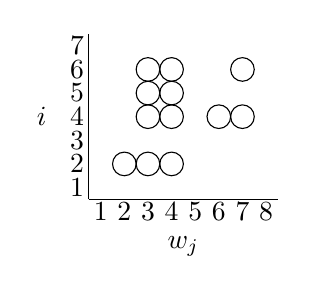
\begin{tikzpicture}[scale=0.3]
\def\rows{8} %number of rows
\def\cols{7} %number of columns
  \draw[-](0,0) -- (\rows,0); %axes
  \draw[-](0,0) -- (0,\cols); 
  \foreach \y in {1,2,...,\cols} %labels
    \draw (-0.5,\y-0.5) node{\y}; 
  \draw (-2,\cols / 2) node{$i$};
  \foreach \x in {1,2,...,\rows}
    \draw (\x-0.5,- 0.5) node{\x};
  \draw (\rows / 2,-2) node{$w_j$}; 
  \foreach \x/\y in {2/2,3/2,4/2,3/4,4/4,6/4,7/4,3/5,4/5,3/6,4/6,7/6} %positions
    \draw (\x-0.5,\y-0.5) circle(0.5);
\end{tikzpicture}
\hspace{2cm}
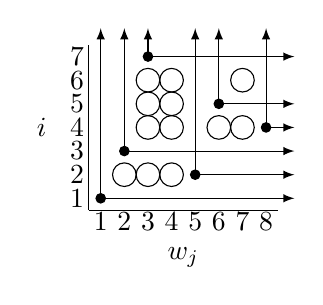
\begin{tikzpicture}[scale=0.3]
\def\rows{8} %number of rows
\def\cols{7} %number of columns
  \draw[-](0,0) -- (\rows,0); %axes
  \draw[-](0,0) -- (0,\cols); 
  \foreach \y in {1,2,...,\cols} %labels
    \draw (-0.5,\y-0.5) node{\y}; 
  \draw (-2,\cols / 2) node{$i$};
  \foreach \x in {1,2,...,\rows}
    \draw (\x-0.5,- 0.5) node{\x};
  \draw (\rows / 2,-2) node{$w_j$}; 
  \foreach \x/\y in {1/1,2/3,3/7,5/2,6/5,8/4} { %dot positions
    \draw[fill=black] (\x-0.5,\y-0.5) circle(0.2);
    \draw[-latex](\x-0.5,\y-0.5) -- (\x-0.5,7.7);
    \draw[-latex](\x-0.5,\y-0.5) -- (8.7,\y-0.5); }
  \foreach \x/\y in {2/2,3/2,4/2,3/4,4/4,6/4,7/4,3/5,4/5,3/6,4/6,7/6} %positions
    \draw (\x-0.5,\y-0.5) circle(0.5);
\end{tikzpicture}
\caption{\label{fig:rothe} The Rothe Diagram $\ID(152869347)$ and the placement of its death rays}
\end{center}
\end{figure}

The \textbf{Lehmer code} of a permutation $L(w)$ is a sequence of integers that counts the number of inversions for each $w_i$ \cite{lehmer1960teaching}.
That is
$$L(w) = (a_1,a_2,...) \in \IN^\infty \text{ such that } a_i = \#\{j > i \colon w_i > w_j\}.$$
The Lehmer code counts the number of bubbles in each row of a Rothe diagram, and it defines a bijection between permutations in $\fS_\infty$ and sequences in $\IN^\infty$ with finitely many nonzero values.
In fact, Lehmer's proved this bijection for $\fS_\infty$ by using the truncated representatives \cite{lehmer1960teaching}.
Thus, for such a sequence $a_1,a_2,...$, there is only one Rothe diagram that has $a_i$ bubbles in the $i$th row for all $i$.
For example, the second and third diagrams in figure \ref{fig:non_rothe_examples} are not Rothe diagrams because the first diagram $\ID(231)$ is the only Rothe diagram with one bubble in the first row, one in the second row, and none in any other row.

\begin{figure}
\begin{center}
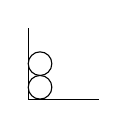
\begin{tikzpicture}[scale=0.3]
\def\rows{3} %number of rows
\def\cols{3} %number of columns
  \draw[-](0,0) -- (\rows,0); %axes
  \draw[-](0,0) -- (0,\cols); 
  \foreach \x/\y in {1/1,1/2} %positions
    \draw (\x-0.5,\y-0.5) circle(0.5);
\end{tikzpicture}
\hspace{1.4cm}
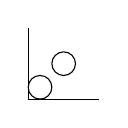
\begin{tikzpicture}[scale=0.3]
\def\rows{3} %number of rows
\def\cols{3} %number of columns
  \draw[-](0,0) -- (\rows,0); %axes
  \draw[-](0,0) -- (0,\cols); 
  \foreach \x/\y in {1/1,2/2} %positions
    \draw (\x-0.5,\y-0.5) circle(0.5);
\end{tikzpicture}
\hspace{1.4cm}
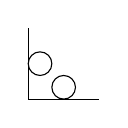
\begin{tikzpicture}[scale=0.3]
\def\rows{3} %number of rows
\def\cols{3} %number of columns
  \draw[-](0,0) -- (\rows,0); %axes
  \draw[-](0,0) -- (0,\cols); 
  \foreach \x/\y in {2/1,1/2} %positions
    \draw (\x-0.5,\y-0.5) circle(0.5);
\end{tikzpicture}
    \caption{$\ID(231)$ and two non-Rothe diagrams}
    \label{fig:non_rothe_examples}
\end{center}
\end{figure}


This is an initial characterization of Rothe diagrams.
Given any finite bubble diagram $D \subset \IZ^+ \times \IZ^+$, we can count the number of bubbles in each row and check that this diagram is equivalent to the Rothe diagram of the permutation with the corresponding Lehmer code.
If not, then $D$ is not a Rothe diagram.
This paper aims to prove other characterizations of Rothe diagrams using conditions on arbitrary diagrams that may provide more insight and connections to other problems.

As we talk about these conditions, it will be useful to have the following equivalent construction of the Rothe diagram $\ID(w)$.
Add dots to $\IZ^+\times \IZ^+$ in the positions $(i,w_i)$ for all $i$.
At each dot, draw two infinite rays coming out of it, one pointing up and one pointing right \cite{knutson2019schubert}.
We call these rays \textbf{\textit{death rays}} and their dot at $(i,w_i)$ a \textbf{\textit{death ray origin}}.
Then, the bubbles in $\ID(w)$ are by definition placed in the cells not touched by a death ray.
Indeed, a bubble is placed in $(i,w_j)$ if and only if $i < j$ and $w_i > w_j$, which is to say $(i,w_j)$ is below $(j,w_j)$ and to the left of $(i,w_i)$, which are the positions of the death ray origins in the $w_j$th column and $i$th row respectively.
See the second diagram in Figure \ref{fig:rothe} for this visualisation.

In the next section we define several properties for bubble diagrams and prove that Rothe diagrams satisfy them.
Then in the following section we see which properties together are sufficient to fully characterize Rothe diagrams.


\section{Properties of Permutation Diagrams}


\begin{definition}
As defined by Assaf \cite{assaf2020demazure}, a diagram $D \subset \IZ^+ \times \IZ^+$ is \textbf{southwest} if for every pair of bubbles $(i_1,w_{j_2}),(i_2,w_{j_1})$ in $D$ with $w_{j_1} < w_{j_2}$ and $i_1 < i_2$, the cell $(i_1,w_{j_1})$ is also in $D$. 
Graphically, a cell with a bubble above it and a bubble to the right of it must also contain a bubble.
\end{definition}

\begin{proposition}
Rothe Diagrams are southwest
\end{proposition}

\begin{proof}
because if we have bubbles $A$ and $B$ at $(i_1,w_{j_2})$ and $(i_2,w_{j_1})$ as in the definition, then there must be a death ray origin to the right of $A$ and one above $B$.
Hence, there must be a bubble at $(i_1,w_{j_1})$, since no death ray touches this position.
\end{proof}


\begin{definition}
For $D \subset \IZ^+ \times \IZ^+$, define \textbf{\textit{row dots}} $R(D) = \{(1,w_1),(2,w_2),...\}$ in $\IZ^+ \times \IZ^+$ such that $(i,w_i)$ is the first position to the right of all the bubbles in the $i$th row that satisfies $w_i \neq w_j$ for all $j < i$.
Similarly, define \textbf{\textit{column dots}} $C(D) = \{(i_1,1),(i_2,2),...\}$ in $\IZ^+\times \IZ^+$ such that $(i_w,w)$ is the first position above all the bubbles in the $w$th column that satisfies $i_w \neq i_v$ for all $v < w$.
We say that a diagram satisfies the \textbf{\textit{dot rule}} and is a \textbf{\textit{dotted diagram}} if $R(D) = C(D)$.
The \textbf{\textit{vertical popping}} rule states that bubbles are not allowed to be placed above row dots, and the \textbf{\textit{horizontal popping}} rule states that bubbles are not allowed to be placed to the right of column dots.
\end{definition}

In Figures \ref{fig:main_dot} and \ref{fig:main_va}, we see which of our examples satisfy these conditions and which do not.
In particular, there are some non-Rothe diagrams that satisfy both the dot rule and the bubble popping rule, implying we will need more conditions to characterize Rothe diagrams.
Now, we prove that Rothe diagrams satisfy both of these rules.

\begin{figure}
\begin{center}
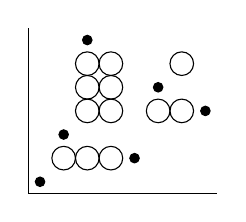
\begin{tikzpicture}[scale=0.3]
\def\rows{8} %number of rows
\def\cols{7} %number of columns
  \draw[-](0,0) -- (\rows,0); %axes
  \draw[-](0,0) -- (0,\cols); 
  \foreach \x/\y in {1/1,2/3,3/7,5/2,6/5,8/4} {%dot positions
    \draw[fill=black] (\x-0.5,\y-0.5) circle(0.2); }
  \foreach \x/\y in {2/2,3/2,4/2,3/4,4/4,6/4,7/4,3/5,4/5,3/6,4/6,7/6} %positions
    \draw (\x-0.5,\y-0.5) circle(0.5);
\end{tikzpicture}
\hspace{1.4cm}
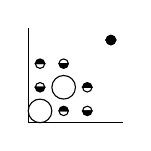
\begin{tikzpicture}[scale=0.3]
\def\rows{4}
\def\cols{4}
  \draw[-](0,0) -- (\rows,0);
  \draw[-](0,0) -- (0,\cols);
  \foreach \x/\y in {1/1,2/2} %circles
    \draw (\x-0.5,\y-0.5) circle(0.5);
  \foreach \x/\y in {2/1,3/2,1/3,4/4}{ %dot-lower empty
    \draw (\x-0.3,\y-0.5) -- (\x-0.7,\y-0.5) arc(180:360:0.2) --cycle;
    \filldraw (\x-0.7,\y-0.5) -- (\x-0.3,\y-0.5)  arc(0:180:0.2) --cycle;} %dot-lower full
  \foreach \x/\y in {1/2,2/3,3/1,4/4}{ %dot-upper full
    \filldraw (\x-0.3,\y-0.5) -- (\x-0.7,\y-0.5) arc(180:360:0.2) --cycle;
    \draw (\x-0.7,\y-0.5) -- (\x-0.3,\y-0.5) arc(0:180:0.2) --cycle;}%dot-upper empty
\end{tikzpicture}
\hspace{1.4cm}
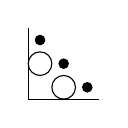
\begin{tikzpicture}[scale=0.3]
\def\rows{3} %number of rows
\def\cols{3} %number of columns
  \draw[-](0,0) -- (\rows,0); %axes
  \draw[-](0,0) -- (0,\cols); 
  \foreach \x/\y in {1/3,2/2,3/1} {%dot positions
    \draw[fill=black] (\x-0.5,\y-0.5) circle(0.2); }
  \foreach \x/\y in {2/1,1/2} %positions
    \draw (\x-0.5,\y-0.5) circle(0.5);
\end{tikzpicture}
  \caption{\label{fig:main_dot}The three example diagrams with the dot condition applied. Here, the middle diagram $D$ fails with $R(D) \neq C(D)$, shown by filled upper and lower semicircles respectively.}
\end{center}
\end{figure}

\begin{figure}
\begin{center}
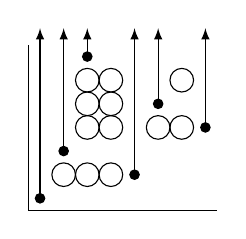
\begin{tikzpicture}[scale=0.3]
\def\rows{8} %number of rows
\def\cols{7} %number of columns
  \draw[-](0,0) -- (\rows,0); %axes
  \draw[-](0,0) -- (0,\cols); 
  \foreach \x/\y in {1/1,2/3,3/7,5/2,6/5,8/4} {%dot positions
    \draw[fill=black] (\x-0.5,\y-0.5) circle(0.2); 
    %vertical lines
    \draw[-latex](\x-0.5,\y-0.5) -- (\x-0.5,7.7); }
  \foreach \x/\y in {2/2,3/2,4/2,3/4,4/4,6/4,7/4,3/5,4/5,3/6,4/6,7/6} %positions
    \draw (\x-0.5,\y-0.5) circle(0.5);
\end{tikzpicture}
\hspace{1.4cm}
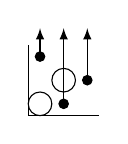
\begin{tikzpicture}[scale=0.3]
\def\rows{3} %number of rows
\def\cols{3} %number of columns
  \draw[-](0,0) -- (\rows,0); %axes
  \draw[-](0,0) -- (0,\cols); 
  \foreach \x/\y in {1/3,3/2,2/1} {%dot positions
    \draw[fill=black] (\x-0.5,\y-0.5) circle(0.2); 
    %vertical lines
    \draw[-latex](\x-0.5,\y-0.5) -- (\x-0.5,3.7); }
  \foreach \x/\y in {1/1,2/2} %positions
    \draw (\x-0.5,\y-0.5) circle(0.5);
\end{tikzpicture}
\hspace{1.4cm}
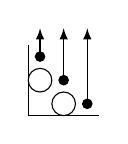
\begin{tikzpicture}[scale=0.3]
\def\rows{3} %number of rows
\def\cols{3} %number of columns
  \draw[-](0,0) -- (\rows,0); %axes
  \draw[-](0,0) -- (0,\cols); 
  \foreach \x/\y in {1/3,2/2,3/1} {%dot positions
    \draw[fill=black] (\x-0.5,\y-0.5) circle(0.2); 
    %vertical lines
    \draw[-latex](\x-0.5,\y-0.5) -- (\x-0.5,3.7); }
  \foreach \x/\y in {2/1,1/2} %positions
    \draw (\x-0.5,\y-0.5) circle(0.5);
\end{tikzpicture}
  \caption{\label{fig:main_va}The three example diagrams with the vertical popping rule applied. Here, the middle diagram is the only one that fails the bubble popping rule.}
\end{center}
\end{figure}

\begin{proposition}\label{pd=>dot}
For a Rothe Diagram $\ID(w)$, we have $R(\ID(w)) = C(\ID(w)) = \{(i,w_i) \in \IZ^+\times \IZ^+\}$.
\end{proposition}

\begin{proof}
First, we find $R(\ID(w))$.
In the first row, we have a death ray origin at $(1,w_1)$ meaning every cell to the left of $(1,w_1)$ is a bubble, and every cell to the right is empty.
Therefore, $(1,w_1)$ is the first position to the right of all the bubbles in the first row, implying $(1,w_1) \in R(\ID(w))$.

Now we induct and assume that $(j,w_j) \in R(\ID(w))$ for all $j < i$.
There is a death ray origin at $(i,w_i)$, meaning there are no bubbles to the right of $(i,w_i)$.
Let $(i,w_j)$ be an empty cell to the left of $(i,w_i)$.
Then the death ray at $(j,w_j)$ must be below this cell, and in particular $j < i$.
By induction we cannot place a row dot in $(i,w_j)$, nor in any empty cell to the left of $(i,w_i)$.
Hence, we must place the row dot in cell $(i,w_i)$, and we conclude that $R(\ID(w)) = \{(i,w_i) \in \IZ^+\times \IZ^+\}$.

Symmetric reasoning proves that $C(\ID(w)) = \{(i,w_i) \in \IZ^+\times \IZ^+\}$ as well.
\end{proof}

Now, whenever we speak of Rothe diagrams we may refer to the death ray origins as dots on a dotted diagram, since they are equivalent.
In particular, all of the facts that are true for death rays apply to dots on a Rothe Diagram.

\begin{proposition}
Rothe diagrams satisfy both the vertical and horizontal popping rules.
\end{proposition}

\begin{proof}
Let $\ID(w)$ be a Rothe Diagram.
By Proposition \ref{pd=>dot}, the equivalent row and column dots are placed in the positions $(i,w_i)$, and these cells correspond to death ray origins.
The death rays prevent bubbles from being placed above the diagram's row dots or to the right of the column dots, and therefore $\ID(w)$ satisfies both popping rules.
\end{proof}


\begin{proposition}
A diagram satisfies the dot rule if and only if it satisfies both popping rules
\end{proposition}

\begin{proof}
If a diagram $D$ satisfies the dot rule, then $R(D) = C(D)$.
Since any row dot is placed to the right of all the bubbles in its row, there are no bubbles to the right of the column dot in the same position.
Similarly, since any column dot is placed above all of the bubbles in its column, there are no bubbles above the row dot in the same position.
Hence, $D$ satisfies both popping rules.

Conversely, assume $D$ satisfies both popping rules.
We prove that $R(D) = C(D)$ by induction on the rows.
In the first row, the row dot is placed immediately after the last bubble in the row.
In fact, the horizontal popping rule requires that there be a bubble in each position to the left of this row dot, for if not then the column dot in this row would be placed to the left of a bubble.
Hence, the column dot must be placed in the position of the row dot here.

Now, assume that row dots and column dots are equivalent for all rows below row $i$.
Let $A$ denote the position of the row dot in row $i$.
By definition, this dot is placed after all of the bubbles in the row and after some number of empty cells, each of which has a row dot below it.
By induction, these are column dots as well, preventing column dots from being placed above these in row $i$.
And since horizontal popping prevents column dots from being placed to the left of any bubbles in row $i$, there are no column dots to the left of $A$.
Lastly, there are no row dots below $A$, so there are no column dots below $A$ by induction.
And there are no bubbles above $A$ by vertical popping, so the column dot in this column must be placed in position $A$, completing the proof.


\end{proof}




\begin{definition}
Consider two procedures for labeling the bubbles in a bubble diagram with numbers.
First, we give the bubbles a \textbf{\textit{horizontal numbering}} where in the $i$th row, we label the bubbles from left to right $i,i+1,i+2,$ and so on.
Second, we give the bubbles a \textbf{\textit{vertical numbering}} where in the $j$th column, we label the bubbles from bottom to top $j,j+1,j+2,$ and so on.
We say a bubble diagram satisfies the \textbf{\textit{numbering condition}} and is an \textbf{\textit{enumerated diagram}} if the horizontal numbering and vertical numbering yield the same labels for each bubble.
\end{definition}

\begin{figure}[ht]
\begin{center}
  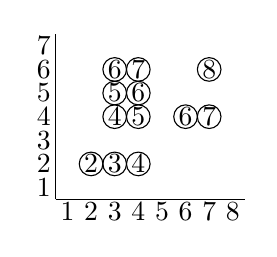
\begin{tikzpicture}[scale=0.3]
\def\rows{8} %number of rows
\def\cols{7} %number of columns
  \draw[-](0,0) -- (\rows,0); %axes
  \draw[-](0,0) -- (0,\cols);
  \foreach \y in {1,2,...,\cols} %labels
    \draw (-0.5,\y-0.5) node{\y}; 
  \foreach \x in {1,2,...,\rows}
    \draw (\x-0.5,- 0.5) node{\x};
  \foreach \x/\y/\n in {2/2/2,3/2/3,4/2/4,3/4/4,4/4/5,6/4/6,7/4/7,3/5/5,4/5/6,3/6/6,4/6/7,7/6/8} %positions
    \draw (\x-0.5,\y-0.5) circle(0.5) node{\n};
\end{tikzpicture}
\hspace{1.5cm}
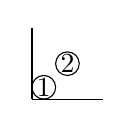
\begin{tikzpicture}[scale=.3]
\def\rows{3} %number of rows
\def\cols{3} %number of columns
  \draw[-](0,0) -- (\rows,0); %axes
  \draw[-](0,0) -- (0,\cols);
  \foreach \x in {1,2} %positions
    \draw (\x-0.5,\x-0.5) circle(0.5) node{\x};
\end{tikzpicture}
\hspace{1.5cm}
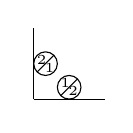
\begin{tikzpicture}[scale=.3]
\def\rows{3} %number of rows
\def\cols{3} %number of columns
  \draw[-](0,0) -- (\rows,0); %axes
  \draw[-](0,0) -- (0,\cols);
  \draw (1/3,5/3) node{\tiny 2};
  \draw (2/3,4/3) node{\tiny 1};
  \draw (4/3,2/3) node{\tiny 1};
  \draw (5/3,1/3) node{\tiny 2};
  \foreach \x/\y in {2/1,1/2}{ %positions
    \draw (\x-0.5,\y-0.5) circle(0.5);
    \draw ({\x-0.5*(1+1/sqrt(2))},{\y-0.5*(1+1/sqrt(2))}) -- ({\x-0.5*(1-1/sqrt(2))},{\y-0.5*(1-1/sqrt(2))});}
\end{tikzpicture}
  \caption{\label{fig:main_number} $\ID(152869347)$ satisfies the numbering condition.
  The second diagram satisfies the condition, but the third does not since its horizontal numbering, shown by the top left numbers in the bubbles, is different from its vertical numbering, shown by the bottom right numbers.}
\end{center}
\end{figure}


\begin{proposition} \label{number_prop}
Permutation diagrams satisfy the numbering condition.
\end{proposition}

\begin{proof}
Consider a bubble $A$ at cell $(i,w_j)$ in a Rothe Diagram $\ID(w)$, which is labeled $n$ by horizontal numbering.
This means there are $n-i$ bubbles to the left of $A$ and therefore $w_j-1 - (n-i)$ empty cells to the left of $A$.
Each of these empty cells corresponds to a dot below it, because no dot can exist to the left of $A$.
So there are $w_j+i-n-1$ dots to the left of the $w_j$th column, beneath row $i$.
Thus, there are $w_j+i-n-1$ empty cells beneath $A$ and therefore $i-1 - (w_j+i-n-1) = n - w_j$ bubbles beneath $A$.
Hence, we also give $A$ the label of $n$ by vertical numbering.
\end{proof}




\begin{definition}
For a given diagram that satisfies the numbering condition, define a \textbf{step-out} to be a pair of bubbles $A$ and $B$ numbered $n$ and $n+1$ respectively, such that $A$ is in position $(i,w)$ and $B$ is in position $(i+k,w+l)$ for positive $k$ and $\ell$.
\end{definition}

A step-out occurs whenever there's a bubble numbered $n$ and a bubble strictly north east numbered $n+1$.
We say that an enumerated diagram is step-out avoiding if no pair of bubbles is a step-out in the diagram.

\begin{proposition}
Rothe diagrams are step-out avoiding.
\end{proposition}

\begin{proof}
Suppose we have a Rothe Diagram $\ID(w)$.
As shown in Proposition \ref{number_prop}, Rothe diagrams are enumerated. 
Take any bubble $A$ numbered $n$ in position $(i,w_j)$ and another bubble $B$ to the right of the $w_j$th column in row $i+k$ for $k > 0$.
We claim that the number in $B$ must be greater than $n+1$.

By the numbering condition, there are $n-i$ bubbles to the left of $A$; call them $C_i,C_{i+1},...,C_{n-1}$.
Let $D \in \{A,C_i,...,C_{n-1}\}$ be one of these bubbles in position $(i,w_{j'})$.
Since permutation diagrams are dotted, there must be a dot above $D$. 
Further, by the dot condition, it must be either above or below the $i+k$th row. 
It cannot be in the $i+k$th as bubble $B$ is already in the $i+k$th row, to the right of the column containing bubble $D$.

If the dot is above, then we have a dot to the right and a dot above position $(i+k,w_j')$ implying the existence of a bubble in this position (\textbf{this should be enough?}).

If the dot is above, then there must be a bubble in position $(i+k,w_{j'})$ since there will be a bubble above and to the right of this position: $B$ is to the right of $(i+k,w_{j'})$, by assumption. 
If there were no bubble in column $w_{j'}$ in or above row $i+k$, then there must be a dot in every row between the highest bubble of the $w_{j'}$ column and the $i+k$ row, by vertical numbering. 
Moreover, vertical numbering requires these dots to occur before column $w_{j'}$. 
Since a dot must be placed somewhere after $B$, not every dot required can be placed. 
Therefore, a bubble is above $(i+k,w_{j'})$. The southwest condition then requires a bubble at this position.


If the dot is below row $i+k$, then position $(i+k,w_{j'})$ must be empty.
Thus, the number of empty cells in the $i+k$th row above any of $A,C_i,...,C_{n-1}$ equals the number of dots above these bubbles and below the $i+k$th row.

This space above these bubbles and below the $i+k$th row has $n-i +1$ columns and $k-1$ rows.
Since dots are never in the same row or column, there must be at most $\min\{n-i+1,k-1\}$ dots in this space.
Now, if $k - 1 \geq n-i + 1$, then our claim is proven since the number in $B$ is at least $k+i \geq n+2$, so assume $\min\{n-i+1,k-1\} = k-1$.
Then there must be at most $k-1$ empty cells in the $i+k$th row above these bubbles.
Then there must be at least $(n-i+1) - (k-1)$ bubbles filling the rest of those positions above the bubbles.
Then the number in $B$ must be at least $i + k + (n-i + 1) - (k-1) = n + 2$.
Hence, the number in $B$ cannot be $n+1$: there are no step-outs in a Rothe diagram.
\end{proof}


\begin{definition}
Assume a column of bubbles in the zero-th column.
\[ (0,w_j) = 1 \; \forall j \in \IZ_+ \]
These bubbles are labelled \textbf{\textit{addendum bubbles}} and are appended to a diagram when considering the rule below. However, these bubbles are not counted towards the total number of bubbles in each row.
\end{definition}

\begin{figure}
\begin{center}
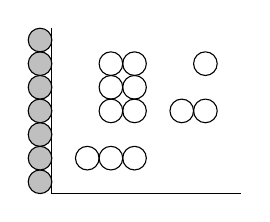
\begin{tikzpicture}[scale=0.3]
\def\rows{8} %number of rows
\def\cols{7} %number of columns
  \foreach \x/\y in {0/1,0/2,0/3,0/4,0/5,0/6,0/7} %addendum bubbles
    \filldraw[fill=black!25,draw=black] (\x-0.5,\y-0.5) circle(0.5);
  \draw[-](0,0) -- (\rows,0); %axes
  \draw[-](0,0) -- (0,\cols); 
  \foreach \x/\y/\n in {2/2/2,3/2/3,4/2/4,3/4/4,4/4/5,6/4/6,7/4/7,3/5/5,4/5/6,3/6/6,4/6/7,7/6/8} %bubbles
    \draw (\x-0.5,\y-0.5) circle(0.5);
\end{tikzpicture}
\hspace{1.4cm}
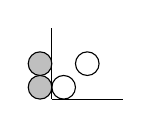
\begin{tikzpicture}[scale=0.3]
\def\rows{3} %number of rows
\def\cols{3} %number of columns
  \foreach \x/\y in {0/1,0/2} %addendum bubbles
    \filldraw[fill=black!25,draw=black] (\x-0.5,\y-0.5) circle(0.5);
  \draw[-](0,0) -- (\rows,0); %axes
  \draw[-](0,0) -- (0,\cols); 
  \foreach \x/\y in {1/1,2/2} %bubbles
    \draw (\x-0.5,\y-0.5) circle(0.5);\end{tikzpicture}
\hspace{1.4cm}
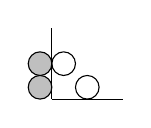
\begin{tikzpicture}[scale=0.3]
\def\rows{3} %number of rows
\def\cols{3} %number of columns
  \foreach \x/\y in {0/1,0/2} %addendum bubbles
    \filldraw[fill=black!25,draw=black] (\x-0.5,\y-0.5) circle(0.5);
  \draw[-](0,0) -- (\rows,0); %axes
  \draw[-](0,0) -- (0,\cols);
  \foreach \x/\y in {2/1,1/2} %bubbles
    \draw (\x-0.5,\y-0.5) circle(0.5);\end{tikzpicture}
  \caption{\label{fig:addendum}The example diagrams with the addendum bubbles shaded.}
\end{center}
\end{figure}


\begin{definition}
The \textbf{\textit{final bubble}} is defined as the last bubble in a row, where all cells afterwards are empty. Final bubbles will be counted with the following function. It returns a $1$ if the final bubble is at the $(i, w_j)$ location and a $0$ otherwise.
\[ R_{(i,w_j)} =  \begin{cases} 
1 & (i,w_j) = 1 \mid (n,w_j) = 0 \quad \forall n > i \\
0 & \text{otherwise}
\end{cases} \]
Since the addendum bubble exists, each row must contain a final bubble.
\end{definition}

\begin{figure}
\begin{center}
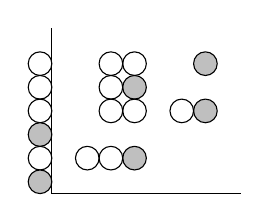
\begin{tikzpicture}[scale=0.3]
\def\rows{8} %number of rows
\def\cols{7} %number of columns
  \foreach \x/\y in {0/2,0/4,0/5,0/6} %positions
    \draw (\x-0.5,\y-0.5) circle(0.5);
  \foreach \x/\y in {0/1,0/3,4/2,7/4,7/6,4/5} %final bubbles
    \filldraw[fill=black!25,draw=black] (\x-0.5,\y-0.5) circle(0.5);
  \draw[-](0,0) -- (\rows,0); %axes
  \draw[-](0,0) -- (0,\cols); 
  \foreach \x/\y in {2/2,3/2,3/4,4/4,6/4,3/5,3/6,4/6} %bubbles
    \draw (\x-0.5,\y-0.5) circle(0.5);
\end{tikzpicture}
\hspace{1.4cm}
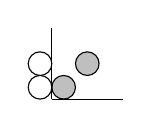
\begin{tikzpicture}[scale=0.3]
\def\rows{3} %number of rows
\def\cols{3} %number of columns
  \draw[-](0,0) -- (\rows,0); %axes
  \draw[-](0,0) -- (0,\cols); 
  \foreach \x/\y in {1/1,2/2} %final bubbles
    \filldraw[fill=black!25,draw=black] (\x-0.5,\y-0.5) circle(0.5);
  \foreach \x/\y in {0/1,0/2} %bubbles
    \draw (\x-0.5,\y-0.5) circle(0.5);
\end{tikzpicture}
\hspace{1.4cm}
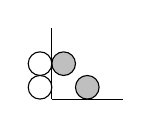
\begin{tikzpicture}[scale=0.3]
\def\rows{3} %number of rows
\def\cols{3} %number of columns
  \draw[-](0,0) -- (\rows,0); %axes
  \draw[-](0,0) -- (0,\cols); 
  \foreach \x/\y in {2/1,1/2} %final bubbles
    \filldraw[fill=black!25,draw=black] (\x-0.5,\y-0.5) circle(0.5);
  \foreach \x/\y in {0/1,0/2} %bubbles
    \draw (\x-0.5,\y-0.5) circle(0.5);
\end{tikzpicture}
  \caption{\label{fig:finals}The three example diagrams with the final bubbles shaded.}
\end{center}
\end{figure}

\begin{definition}
Consider a bubble $(i, w_j) = 1$ that is succeeded by $n$ empty cells 
\[(i+k, w_j) = 0 \quad \forall k \leq n, \quad k,n \in \IZ_+ \]
and a bubble after these empty cells $(i+(n+1), w_{j}) = 1$. Take a box bounded by the two aforementioned bubbles and the bottom of the diagram. Remove the rightmost column and topmost row.
\[ \mathcal{B}_{(i+(n+1), w_{j})} = ([i,i+n], [1,w_{j-1}]) \]
%\[ \mathcal{B}_{(i+(n+1), w_{j})} = [(i, w_{j-1}),(i,1)] \times [(i,w_{j-1}), (i+n, w_{j-1})] \]
The \textbf{\textit{empty cell gap}} rule states there are exactly $n$ final bubbles contained within box $\mathcal{B}$.
\end{definition}

\begin{figure}
\begin{center}
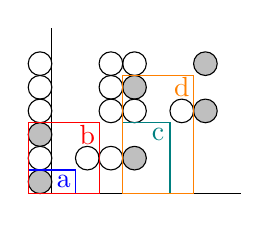
\begin{tikzpicture}[scale=0.3]
\def\rows{8} %number of rows
\def\cols{7} %number of columns
  \foreach \x/\y in {0/2,0/4,0/5,0/6} %positions
    \draw (\x-0.5,\y-0.5) circle(0.5);
  \foreach \x/\y in {0/1,0/3,4/2,7/4,7/6,4/5} %final bubbles
    \filldraw[fill=black!25,draw=black] (\x-0.5,\y-0.5) circle(0.5);
  \draw[-](0,0) -- (\rows,0); %axes
  \draw[-](0,0) -- (0,\cols); 
  \foreach \x/\y in {2/2,3/2,3/4,4/4,6/4,3/5,3/6,4/6} %bubbles
    \draw (\x-0.5,\y-0.5) circle(0.5);
  %rectangles
  \draw[draw=blue] (-1,0) rectangle ++(2,1);
    \draw (0.5,0.5) node{\color{blue} a};
  \draw[draw=red] (-1,0) rectangle ++(3,3);
    \draw (1.5,2.5) node{\color{red} b};
  \draw[draw=teal] (3,0) rectangle ++(2,3);
    \draw (4.5,2.5) node{\color{teal} c};
  \draw[draw=orange] (3,0) rectangle ++(3,5);
    \draw (5.5,4.5) node{\color{orange} d};
\end{tikzpicture}
\hspace{1.4cm}
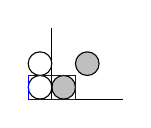
\begin{tikzpicture}[scale=0.3]
\def\rows{3} %number of rows
\def\cols{3} %number of columns
  \draw[-](0,0) -- (\rows,0); %axes
  \draw[-](0,0) -- (0,\cols); 
  \foreach \x/\y in {1/1,2/2} %final bubbles
    \filldraw[fill=black!25,draw=black] (\x-0.5,\y-0.5) circle(0.5);
  \foreach \x/\y in {0/1,0/2} %bubbles
    \draw (\x-0.5,\y-0.5) circle(0.5);
  \draw[draw=blue] (-1,0) rectangle ++(2,1); %rectangle
\end{tikzpicture}
\hspace{1.4cm}
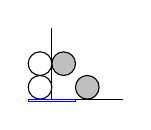
\begin{tikzpicture}[scale=0.3]
\def\rows{3} %number of rows
\def\cols{3} %number of columns
  \draw[-](0,0) -- (\rows,0); %axes
  \draw[-](0,0) -- (0,\cols); 
  \foreach \x/\y in {2/1,1/2} %final bubbles
    \filldraw[fill=black!25,draw=black] (\x-0.5,\y-0.5) circle(0.5);
  \foreach \x/\y in {0/1,0/2} %bubbles
    \draw (\x-0.5,\y-0.5) circle(0.5);
  \draw[draw=blue] (-1,0) rectangle ++(2,-.1); %rectangle
\end{tikzpicture}
  \caption{\label{fig:ecg_main}The main diagram satisfies the empty cell gap rule is satisfied. 
  Box $a = \mathcal{B}_{(2, 2)}$ is generated by a gap of length one and contains one final bubble. 
  Box $b = \mathcal{B}_{(4, 3)}$, box $c = \mathcal{B}_{(4, 6)}$, and box $d = \mathcal{B}_{(7, 7)}$ have two, one, and two final bubbles (respectively) and also corresponding gaps of length two, one, and two (respectively). 
  Two of the six empty cell gap boxes are omitted -- $\mathcal{B}_{(5, 3)}$ and $\mathcal{B}_{(6, 3)}$ -- for readability, but it should be noted that these two gaps also satisfy the empty cell gap rule.
  The middle diagram only requires one box $\mathcal{B}_{(2,2)}$ to be checked, and it does satisfy the empty cell gap rule.
  Finally, the diagram on the right also only creates one box $\mathcal{B}_{(1,2)}$. 
  This box has height zero and so cannot contain the single final required by the gap. Therefore this graph does not fulfill the empty cell gap rule.}
\end{center}
\end{figure}

\begin{proposition}
Permutation diagrams satisfy the empty cell gap rule.
\end{proposition}

\begin{proof}
\textbf{todo: indexing fix}
Assume a bubble in the cell $(i_1,w_{j})$ and $(i_2+1, w_{j})$, where the $((i_2+1) - i_1) = n$ cells in between are all empty. The permutation diagram requires exactly $n$ death rays to begin between the $i_1$ and $i_2+1$ columns and below the $w_{j}$ row. Given that the $(i_1,w_{j})$ bubble exists,  a death ray cannot be located in the $i_1$ column below the $w_{j}$ row. Therefore, for every death ray beginning between the $i_1$ and $i_2+1$ columns, a final bubble is contained in the $i_1$ to $i_2-1$ column range. So, the empty cell gap rule is satisfied by permutation diagrams.
\end{proof}

\section{Conditions for Building Permutation Diagrams}

\begin{theorem}
A bubble diagram satisfies the bubble popping and empty cell gap rules if and only if it is a permutation bubble diagram.
\end{theorem}

\begin{proof}
Arbitrary bubble diagrams that satisfy the cell gap and bubble popping rules are unique, given a number of bubbles for each row. 
In order to prove that these two rules determine a unique bubble diagram (up to rows), we use induction on those rows, starting with the leftmost bubble in each row and moving right. 
We also make use of the addendum column in this proof.
\\ \par
\textit{Row $1$:} If there are no bubbles in row one $(i,w_1) = 0 \; \forall j \in \IZ_+$, then the row is all empty cells (besides the addendum bubble). 
If $\sum_{i=1}^{\infty} (i,w_1) = m, \; m > 0$, then the row cannot start with any number of empty cells. 
These empty cells would violate the empty cell gap rule (given the addendum bubble). 
There are no rows below the first row, so any gap will necessary have an insufficient number of bubbles. 
The same argument applies to the rest of the row. 
Any gaps in the first row of bubbles are prevented by the lack of lower final bubbles. 
Therefore, for a given number of bubbles, row one is unique.
\\ \par
\textit{Row $k+1$:} If there are no bubbles in row $k+1$
\[ (i,w_{k+1}) = 0 \; \forall i \]
then the row is full of empty cells (besides the addendum bubble). 
On the other hand, if $\sum_{i=1}^{\infty} (i,w_{k+1}) = m, \; m > 0$, start with the leftmost column, i.e. the zeroth column. 
We know by definition the addendum it is always filled. 
Take cell $c = (i_2+1,w_{k+1})$. 
Either it is preceded by a bubble, or it is preceded by an empty cell. Take each of these scenarios in turn.
\\ \par
First, assume that cell $c$ is directly preceded by a bubble $(i_2,w_{k+1}) = 1$. 
If the bubble popping rule applies, the cell must be empty. 
If the bubble popping rule doesn't apply, assume for contradiction that cell $c$ is left empty. 
Then, for cell $d_0 = (i_2+2,w_{k+1})$ to be a filled with a bubble, there must be exactly one final bubble in box $\mathcal{B}_{d_0}$, fulfilling the empty cell gap rule. 
If $\mathcal{B}_{d_0}$ does have a final bubble, then that final bubble could not be in the $i_2$ column. 
If that final bubble was in the $i_2$ column, then the bubble popping rule would apply to cell $c$. 
So, the final bubble must be in box $\mathcal{B}_{d_0}$'s other column, the $i_2+1$ column. 
A final bubble in this column, however, means that cell $d_0$ must be empty.
\\ \par
Next, take cell $d_{a+1} = (i_2+(a+3),w_{k+1}), \; a \geq 0$. 
There must be $a+2$ final bubbles in the $\mathcal{B}_{d_{a+1}}$ box for $d_{a+1}$ to fulfill the empty cell gap rule. 
For each column between $i_2$ and $i_2+(a+3)$, the final bubble count of box $\mathcal{B}_{d_{a+1}}$ can increase by $n$. 
However, the bubble popping rule would correspondingly add $n$ dots. 
Since the first empty cell $d_0$ did not have a final bubble, box $\mathcal{B}_{d_{a+1}}$ will always be at least one final bubble short when the bubble popping rule is fulfilled. 
Therefore, there are bubbles left to place but all remaining locations in the row do not fulfill one or both of the rules. 
So, by contradiction, if the bubble popping rule doesn't apply when a cell $c$ is preceded by a bubble, then $c$ must be a bubble. 
Bubble locations for an arbitrary diagram are then uniquely determined when those bubbles are placed directly after other bubbles.
\\ \par
Conversely, take a cell $c = (i,w_j)$ preceded by at least one empty cell. 
Assume without loss of generality that $c$ is preceded by $n$ empty cells.
\[(i-k,w_j) = 0 \quad \forall k \in \IZ_+, \; k \leq n \]
If $c$ fulfills the empty cell gap rule, then -- by the logic presented above -- a bubble must be placed in cell $c$. 
Otherwise, the empty cell gap rule will never again be fulfilled (or fulfilled only in the case where the bubble popping rule is broken), and the row will not have enough bubbles in it. 
On the other hand, assume cell $c$ does not satisfy the empty cell gap rule. 
Note that the gap must have originally been created because of an application of the bubble popping rule. 
Then, at least one final bubble is in the box $\mathcal{B}_c$ created by this gap. 
If there are $m$ final bubbles in the $i-n$ column, the gap must (by the bubble popping rule) be at least $m$ empty cells long. 
However, if more final bubbles appeared after the $i-n$ column or if $m<n$, then box $\mathcal{B}_c$ will still have too many final bubbles and not enough gaps. 
Since the bubbles on a graph are finite, at some point the number of final bubbles will stop increasing. 
Then, there exists some number of gaps which will equal the number of final bubbles in box $\mathcal{B}$. 
Therefore, there is always a unique cell after a gap for a bubble. 
Before this cell, there will be too many empty cells as compared to final bubbles. 
After this cell, there will always be insufficient final bubbles or a contradiction with the bubble popping rule. 
%Note that it is impossible for a graph to have too many required gaps from the bubble popping rule and not enough final bubbles for the empty cell gap rule. 
So, the two rules can always create a unique bubble diagram.

We know that for any Lehmer code, there exists a corresponding permutation with a unique number of bubbles up to rows by Proposition \ref{pd=>dot}. 
Lehmer codes give the number of bubbles in each row of the corresponding Rothe Diagram.

Given a number of bubbles for each row, the Lehmer code tells us that a unique permutation diagram exists. 
As just proven, a unique bubble diagram that satisfies the empty cell gap and bubble popping rules also exists. 
Since these two rules are satisfied by permutation diagrams, the diagram generated by these two rules must be identical to the permutation diagram.
\end{proof}

\begin{theorem}
A bubble diagram satisfies the dot condition and the numbering condition if and only if it is a permutation bubble diagram.
\label{thm:DC+NC}
\end{theorem}

\begin{proof}
Consider an arbitrary bubble diagram that satisfies the dot and numbering conditions.
Place the dots on the diagram and let $(1,w_1),(2,w_2),...$ denote their positions.
In fact, since the dots are never in the same column, we are able to refer uniquely to the $w_j$th column and the $(i,w_j)$th position without confusion.
We claim that a bubble is placed in the position $(i,w_j)$ exactly when $i < j$ and $w_i > w_j$, which shows that this diagram is a permutation bubble diagram corresponding to the permutation $w_1,w_2,...$

Assume there is a bubble in position $(i,w_j)$.
By the dot condition there must be a dot above and a dot to the right of this position.
The dot above is in position $(j,w_j)$ meaning $i < j$, and the dot to the right is in position $(i,w_i)$ meaning $w_i > w_j$.

Conversely, consider a position $(i,w_j)$ such that $i < j$ and $w_i > w_j$.
We claim there must be a bubble in any such position, and we prove it by induction on $i$.
In the base case, the positions to the left of the dot at $(1,w_1)$ are the only ones to satisfy the assumption.
And indeed we must place a bubble in each of these positions.
For if not, then using the vertical dot-placing method, we would place a dot in a position to the left of $(1,w_1)$, violating the dot condition.

Now, let's assume we've shown that there is a bubble in every position $(i,w_j)$ such that $i < j$ and $w_i > w_j$ for all $i < I$, for some $I > 1$.
Consider a position $(I,w_j)$ with $I < j$ and $w_I > w_j$, and assume there is no bubble in this position.
Then, there must be a bubble $A$ in position $(I,w_{j'})$ for some $w_j < w_{j'} < w_{I}$, for if not then the horizontal method would place a dot in a different position than $(I,w_I)$ contradicting the dot condition.
There must be a dot above $A$ by the dot condition.
Then by induction, we see that the number of bubbles below $A$ is equal to the number of dots to the right of the $w_{j'}$th column and below the $I$th row, call this value $d$.
Then by the numbering condition, we would label $A$ with the number $w_{j'} + d$ when counting vertically.

However, we get something different if we count horizontally.
There are $I - 1 - d$ dots to the left of the $w_{j'}$th column and below the $I$th row, none of which are in the $w_j$th column.
That means there are at least $I - d$ empty cells to the left of $A$, since $(I,w_j)$ is empty.
If we count horizontally, then we would label $A$ with the number
$$I + \#\{\text{positions to the left of }A\} - \#\{\text{empty positions to the left of }A\}.$$
This is at most
$$I + (w_{j'} - 1) - (I - d) = w_{j'} + d - 1,$$ 
which is strictly less than our previous label.
This contradicts the numbering condition and our assumption that $(I,w_j)$ contains no bubble must be false.
Hence, this diagram is in fact the permutation bubble diagram for the permutation $w_1,w_2,...$, showing that any diagram satisfying the dot and numbering conditions is a permutation diagram.
\end{proof}


\begin{proposition}
A bubble diagram satisfies the dot condition and the southwest condition if and only if it is a permutation bubble diagram.
\end{proposition}

\begin{proof}
The proof is identical to the proof of Theorem \ref{thm:DC+NC}, except the inductive step is easier.
In this step, we consider a position $(i,w_j)$ such that $i < j$ and $w_i > w_j$, and we wish to show that there must be a bubble in this position by induction on $i$.
The base case is proven, and now we assume we've shown the claim for all $i < I$, for some $I > 1$.
Consider a position $(I,w_j)$ with $I < j$ and $w_I > w_j$, and assume there is no bubble in this position.
As we saw before, there must be a bubble $A$ in position $(I,w_{j'})$ for some $w_j < w_{j'} < w_I$, and similarly there must be a bubble $B$ in position $(i',w_j)$ for some $I < i' < j$.
Then the southwest condition requires a bubble be placed in position $(I,w_j)$.
\end{proof}

\begin{theorem}
A diagram is a permutation diagram if and only if it is enumerated and step-out avoiding.
\end{theorem}

\begin{proof}
Given a non negative sequence $a_1,a_2,...$ with finitely many nonzero elements, we claim there exists a unique enumerated step-out avoiding diagram that has $a_i$ bubbles in the $i$th row for all $i$.
There is also a unique permutation diagram that has $a_i$ bubbles in the $i$th row for all $i$.
And since the permutation diagram is enumerated and step-out avoiding, these must be the same diagram.

To show the claim, we construct the enumerated step-out avoiding diagram row by row in the only way possible.
The first row is determined by the numbering condition alone and we fill in the first $a_1$ positions with bubble.
Now assume the first $i-1$ rows have been constructed such that the numbering condition and step-out avoidance are satisfied.
We have $a_i$ bubbles to place in the $i$th row.
If $a_i = 0$ we are done, and if not, then the first bubble must be numbered $i$, so we must place this bubble in a column whose uppermost bubble so far is numbered $i-1$.
If there are multiple options, then we must choose the left-most option, for if not, then the left-most option will form a step-out with the newly placed bubble.
This logic continues for every bubble in this row, and we get a unique placement.
\end{proof}

Note, we can easily define the numbering condition and the step-out avoiding condition for a collection of ``fixed" columns who have yet to be put in an actual column position yet.




\bibliographystyle{plain}
\bibliography{refs}

\end{document}